\subsection{Delimitation}
Ground handling is a very big area and to cover it all would therefore be to big for this project and therefore some delimitation needs to be done.
When visiting Aalborg airport we got a look inside how different areas of ground handling are organized and as seen in figure \ref{AALStructure} the COO (Kim Bermann), the person we interviewed during our visit, is the one having absolute most ground handling services. Since Kim is the operational leader we have choose only to focus on his field therefore delimitating food and beverage, being the only ground handling task Kim is not in charge of, although we will dealing indirectly with communication.

\begin{figure}[H]
\centering
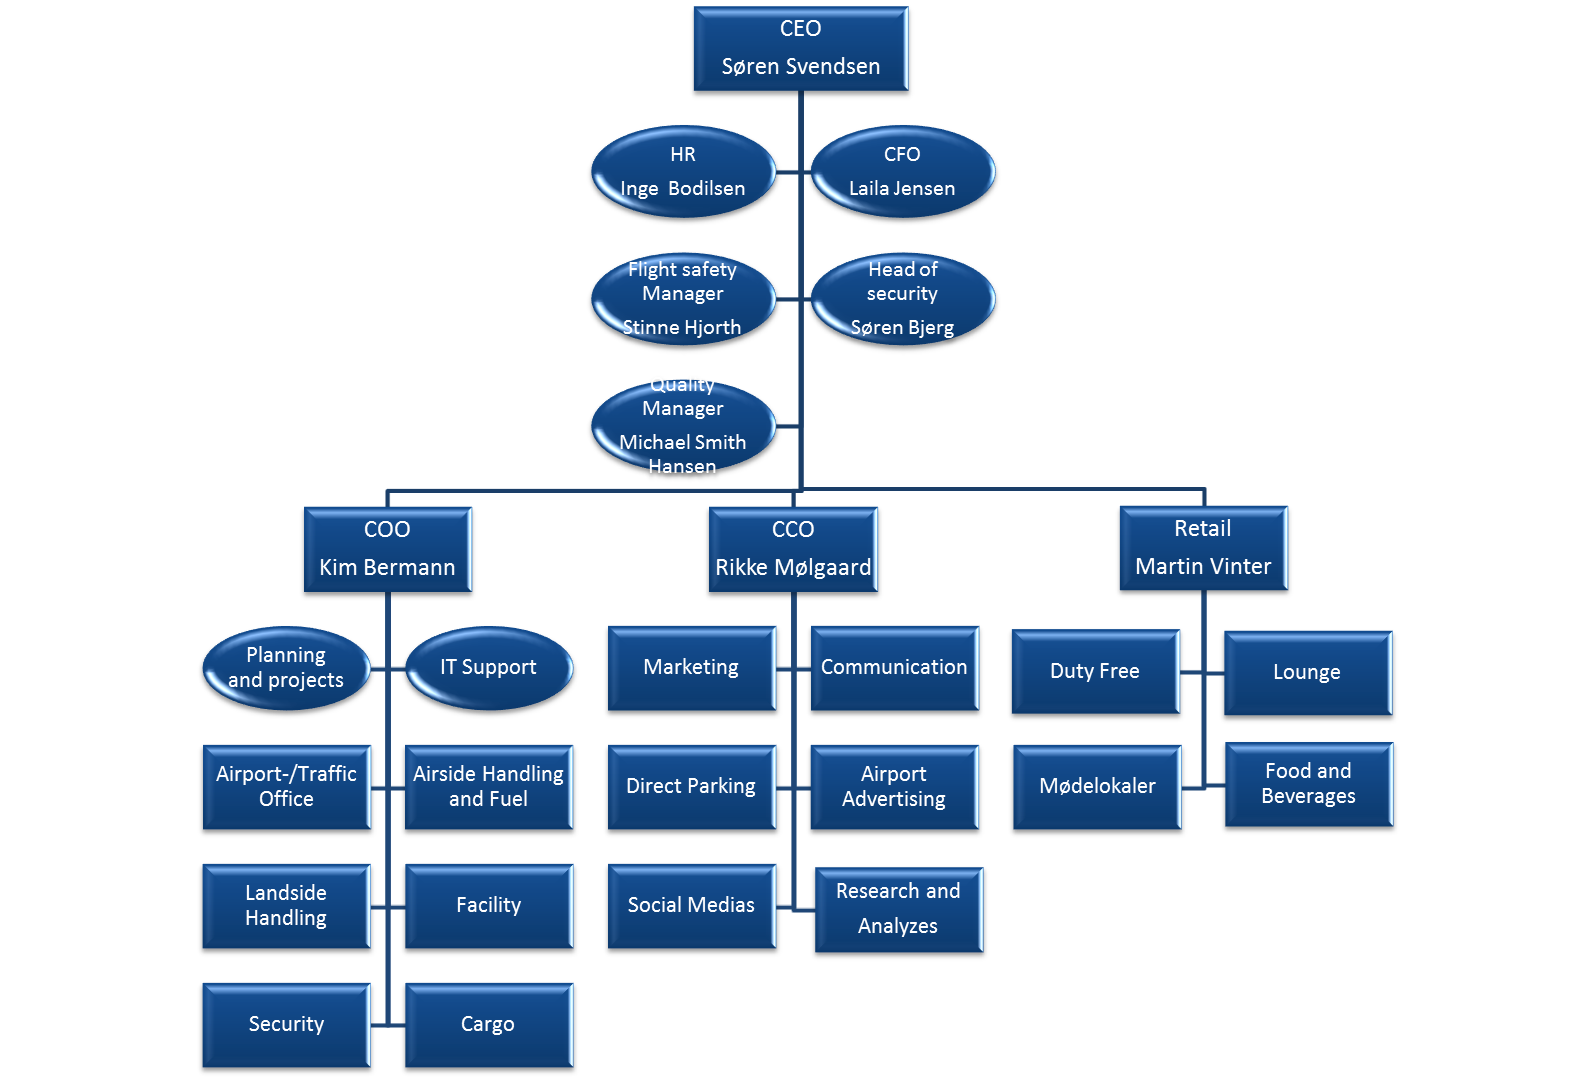
\includegraphics[width=\textwidth]{Grafik/AALStructure}
\caption{The organisational structure of Aalborg Airport.}
\label{AALStructure}
\end{figure}

The largest field of the ground handling is what is done to the airplane on the apron, therefore we have decided to delimit all ground handling task not being done on the apron with the exception of cargo and luggage, thereby delimitating check-in, security and taxiing of aircraft, and ofcause everything done in-flight. These are the areas left:

\begin{itemize}
\item Freight
\item Fueling
\item Cleaning
\item Catering
\item Pushback
\item Passengers
\item Power
\item Bridges/stairs
\item Lavatories
\item Water
end{itemize}